\chapter{Case Studies}

\begin{note}{Reference}
    Yoav Goldberg, Neural Network Methods for Natural Language Processing.\cite{goldberg2017neural}
    Part II, Chapter 7.
\end{note}

After discussing the different sources of information available for deriving features from natural language text, we will now explore examples of concrete NLP classification tasks, and suitable features for them.
Of course, modern language models may achieve very high performance on these tasks, but they may also be overkill. In this chapter, we will see features that are useful to build simpler yet very powerful models.
When talking about performance, we should always keep in mind the related costs: large language model are often huge and require very powerful runtimes.

\section{Document classification}
In this section, we discuss features that are suitable for document classification tasks.

\subsection{Language identification}
We are given a text and want to classify it into one of a fixed set of languages. Bag-of-letter-bigrams is a very strong feature representation for this task.

\begin{example}{}
    For language identification, the \qi{bag-of-letter-bigrams} representation captures statistical patterns of consecutive letter pairs. Consider two texts: \qi{The quick brown fox jumps over the lazy dog} (English) and \qi{La veloce volpe marrone salta sul pigro cane} (Italian).
    Extracting and counting letter bigrams (ignoring spaces and punctuation) yields distinct distributions: English texts often contain bigrams like \qi{th}, \qi{he}, or \qi{qu}, while Italian texts feature bigrams like \qi{il}, \qi{ve}, or \qi{ce}. These bigram counts serve as features for a classifier, enabling it to distinguish between languages based purely on statistical patterns.
\end{example}

\subsection{Topic classification}
We are given a text and need to classify it into one of a predefined set of topics. If we do not have many training examples, it may be a good idea to consider lemmas or stems rather than entire words. When using BOW, the TF-IDF encoding is very powerful. However, a learning algorithm is often capable of coming up with the weighting on its own.

\subsection{Authorship attribution}
In the authorship attribution task, we are given a text and need to infer the identity of its author from a fixed set of possible authors, or other characteristics of the author of the text, such as their gender, their age, or their native language.

The kind of information used to solve this task is very different from that of topic classification---the clues are subtle and involve stylistic properties of the text rather than content words. For this reason, we may want to adopt features that focus on the structure rather than the content. We can do so by considering POS and function words, namely words like \textit{on, of, before}, as well as pronouns to capture the author's style. A good approximation of function words is the top-300 most frequent words in a large corpus.

\begin{example}{}
For instance, consider the following sentences \qi{The cat sat on the mat.} and \qi{Upon the mat, the cat did sit.}
While both convey similar content, their stylistic differences—such as the use of \qi{on} vs. \qi{upon}, or the presence of the auxiliary \qi{did}—can serve as features. 
These features help distinguish authors based on their unique stylistic patterns rather than the topics they discuss.
\end{example}

\section{Word in context}


\subsection{POS tagging}
In the parts-of-speech tagging task, we are given a sentence and need to assign the correct part-of-speech to each word in the sentence. The POS tags belong to a predefined set; for this example, assume we will be using the tagset of the Universal Treebank Project (UTP, 2017), containing 17 tags: 
\begin{itemize}
    \item \qi{ADJ}: Adjective, describes a noun. Example: \qi{lazy} in \qi{the lazy dog}.
    \item \qi{ADP}: Adposition (preposition or postposition). Example: \qi{in} in \qi{in the house}.
    \item \qi{ADV}: Adverb, modifies a verb, adjective, or other adverb. Example: \qi{quickly} in \qi{She ran quickly.}
    \item \qi{AUX}: Auxiliary verb, helps express tense, mood, or voice. Example: \qi{is} in \qi{She is running.}
    \item \qi{CONJ}: Coordinating conjunction, connects words or phrases. Example: \qi{and} in \qi{cat and dog}.
    \item \qi{DET}: Determiner, introduces a noun. Example: \qi{the} in \qi{the cat}.
    \item \qi{INTJ}: Interjection, expresses emotion. Example: \qi{Oh!} in \qi{Oh! That's surprising.}
    \item \qi{NOUN}: Noun, names a person, place, or thing. Example: \qi{dog} in \qi{the dog barks}.
    \item \qi{NUM}: Numeral, represents a number. Example: \qi{three} in \qi{three cats}.
    \item \qi{PART}: Particle, often part of phrasal verbs or idioms. Example: \qi{up} in \qi{give up}.
    \item \qi{PRON}: Pronoun, replaces a noun. Example: \qi{she} in \qi{She is happy.}
    \item \qi{PROPN}: Proper noun, names a specific entity. Example: \qi{John} in \qi{John is here.}
    \item \qi{PUNCT}: Punctuation, marks the end of a sentence or separates clauses. Example: \qi{.} in \qi{Hello.}
    \item \qi{SCONJ}: Subordinating conjunction, introduces a dependent clause. Example: \qi{because} in \qi{She left because she was tired.}
    \item \qi{SYM}: Symbol, represents a non-linguistic symbol. Example: \qi{\$} in \qi{\$100}.
    \item \qi{VERB}: Verb, expresses an action or state. Example: \qi{run} in \qi{She runs fast.}
    \item \qi{X}: Other, for words that don't fit into the above categories. Example: \qi{abc} in \qi{the word abc}.
\end{itemize}

Part-of-speech tagging is usually modeled as a structured task---the tag of the first word may depend on the tag of the third one---but it can be approximated quite well by classifying each word in isolation into a POS-tag based on a window of two words to each side of the word. If we tag the words in a fixed order, for example from left to right, we can also condition each tagging prediction on tag predictions made on previous tags.

\begin{example}{}
    Consider the sentence:
    \qi{The lazy dog slept.}
    The corresponding POS tags using the UTP tagset are:
    \qi{DET ADJ NOUN VERB PUNCT}
\end{example}

However, we will see that bidirectional recurrent networks (biRNN) achieve better performance by considering both directions.

\subsection{Named entity recognition}
In the named-entity recognition (NER) task, we are given a document and need to find named entities such as Milan, John Smith, McCormik Industries, and Paris, as well as to categorize them into a predefined set of categories such as LOCATION, ORGANIZATION, PERSON, or OTHER.

\begin{note}{}
    Note that this task is context-dependent, as Milan can be a location (the city) or an organization (a sports team, \qi{Milan played against Barcelona Wednesday evening}), and Paris can be the name of a city or a person.
\end{note}{}

NER is usually modeled as a sequence tagging task like POS tagging. In particular, in NER, we use BIO-encoded tags: 
\begin{itemize}
    \item \qi{O}: Outside, not part of any named entity. Example: \qi{The} in \qi{The man lives in Rome.}
    \item \qi{B-PER}: Beginning of a person name. Example: \qi{John} in \qi{John Doe works here.}
    \item \qi{I-PER}: Inside (continuation) of a person name. Example: \qi{Doe} in \qi{John Doe works here.}
    \item \qi{B-LOC}: Beginning of a location name. Example: \qi{New} in \qi{New York is a city.}
    \item \qi{I-LOC}: Inside (continuation) of a location name. Example: \qi{York} in \qi{New York is a city.}
    \item \qi{B-ORG}: Beginning of an organization name. Example: \qi{Google} in \qi{Google LLC was founded in 1998.}
    \item \qi{I-ORG}: Inside (continuation) of an organization name. Example: \qi{LLC} in \qi{Google LLC was founded in 1998.}
    \item \qi{B-MISC}: Beginning of a miscellaneous entity. Example: \qi{Titan} in \qi{Titan is a moon of Saturn.}
    \item \qi{I-MISC}: Inside (continuation) of a miscellaneous entity. Example: \qi{Saturn} in \qi{Titan is a moon of Saturn.}
\end{itemize}

\begin{example}{}
    \qi{John Smith, president of McCormik Industries visited his niece Paris in Milan, reporters say.} should produce the output \qi{John/B-PER Smith/I-PER ,/O president/O of/O McCormik/B-ORG Industries/I-ORG visited/O his/O niece/O Paris/B-PER in/O Milan/B-LOC.}
\end{example}

So, given the analogies, the set of features for this task is quite similar to the POS tagging one.

\subsection{Preposition sense disambiguation}
Prepositions, words like \textit{on, in, with}, and \textit{for}, serve for connecting predicates with their arguments and nouns with their prepositional modifiers. Prepositions are very common and also very ambiguous. For example, consider the word \qi{for}: 
\begin{itemize}
    \item[a)] \qi{we went there for lunch}
    \item[b)] \qi{he paid for me}
    \item[c)] \qi{we ate for two hours}
    \item[d)] \qi{he would have left for home, but it started raining}
\end{itemize}

In (a), ``for'' indicates purpose, in (b) a beneficiary, in (c) a duration, and in (d) a location. 
In order to fully understand the meaning of a sentence, one should arguably know the correct senses of the prepositions within it. 
The preposition-sense disambiguation task deals with assigning the correct sense to a preposition in context, from a finite inventory of senses.

Linguists say that to understand a preposition, we must look at its verb (called governor) and its object. We could use some heuristics or a dependency parser or both.
For example, in (a), the governor is \qi{went} and the object \qi{lunch}, so the most likely meaning of \qi{for} is purpose.
Similarly, in (c), the governor is \qi{ate} and the object is \qi{hours}, suggesting that \qi{for} is indicating a duration.

\section{Relation between two words in context}
\subsection{Arc-factored parsing}
In the dependency parsing task, we are given a sentence and need to return a syntactic dependency tree over it. Each word is assigned a parent word, except for the main word of the sentence whose parent is a special \texttt{*ROOT*} symbol.

One approach to modeling the task is the arc-factored approach, where each of the possible $n^{2}$ word-word relations (arcs) is assigned a score independent of the others, and then we search for the valid tree with the maximal overall score. The score assignment is made by a trained scoring function \texttt{ARCSCORE($h$, $m$, sentence)}, receiving a sentence as well as the indices $h$ and $m$ of two words within it that are considered as candidates for attachment ($h$ is the index of the candidate head-word and $m$ is the index of the candidate modifier).

As features, we should use words and their POS tags. One could replace words with their embeddings. Another useful feature is the signed distance ($|h - m|$) between the head and the modifier.

\begin{example}{}
In the arc-factored parsing approach, we consider the sentence \qi{The cat chased the mouse.} and assign part-of-speech (POS) tags to each word:

\begin{center}
\begin{tabular}{c c c}
\hline
Index & Word & POS Tag \\
\hline
0 & The & DET \\
1 & cat & NOUN \\
2 & chased & VERB \\
3 & the & DET \\
4 & mouse & NOUN \\
5 & . & PUNCT \\
\end{tabular}
\end{center}

If we train correcly the scoring function, then the highest-scoring valid tree for this sentence should be:

\begin{center}
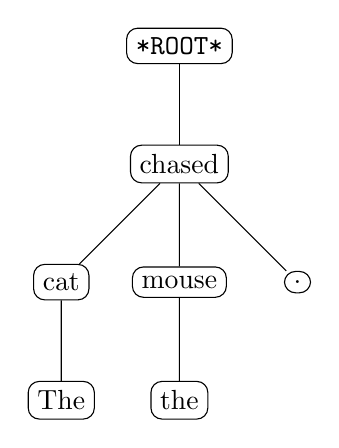
\begin{tikzpicture}[
    level distance=1.5cm,
    level 1/.style={sibling distance=3cm},
    level 2/.style={sibling distance=1.5cm},
    every node/.style={draw, rectangle, rounded corners, thin}
]
\node {\texttt{*ROOT*}}
    child { node {chased}
        child { node {cat}
            child { node {The} }
        }
        child { node {mouse}
            child { node {the} }
        }
        child { node {.} }
    };
\end{tikzpicture}
\end{center}
Note that, in standard dependency parsing, punctuation marks (like the final dot) are typically included in the dependency tree. They are usually attached to the head of the clause or sentence they terminate.
\end{example}